\documentclass[aspectratio=169,10pt]{beamer}

\usetheme{Madrid}
\usecolortheme{seahorse}

\usepackage{amsmath}
\usepackage{amssymb}
\usepackage{amsfonts}
\usepackage{mathtools}
\usepackage{graphicx}
\usepackage{listings}
\usepackage{xcolor}
\usepackage{hyperref}

% Code listing style
\lstset{
    basicstyle=\ttfamily\scriptsize,
    commentstyle=\color{green!50!black}\itshape,
    keywordstyle=\color{blue}\bfseries,
    numbers=left,
    numberstyle=\tiny\color{gray},
    frame=single,
    breaklines=true,
    breakatwhitespace=true,
    showstringspaces=false,
    language=Python
}

% Theorem styles for Beamer
\newtheorem{defn}{Definition}
\newtheorem{thm}{Theorem}
\newtheorem{lem}{Lemma}
\newtheorem{prop}{Proposition}
\newtheorem{corol}{Corollary}
\newtheorem{ex}{Example}

% Graphics path
\graphicspath{{figures/}}

% Fonts
\usepackage{helvet}

% Set footline
\setbeamertemplate{footline}[frame number]

% Title and author
\title{Vector Spaces \& Functional Analysis}
\subtitle{Pathak Chapter 5c: Pages 517--538}
\author{Nonlinear Analysis and Fixed Point Theory}
\date{\today}

\begin{document}

% ============================================================================
% Title Slide
% ============================================================================

\begin{frame}
  \titlepage
  \begin{center}
    \small An Introduction to Nonlinear Analysis and Fixed Point Theory (2018)
  \end{center}
\end{frame}

% ============================================================================
% Table of Contents
% ============================================================================

\begin{frame}[allowframebreaks]{Outline}
  \tableofcontents
\end{frame}

% ============================================================================
% Section 1: Banach Spaces
% ============================================================================

\section{Banach Spaces}

\begin{frame}{Banach Spaces: Definition}
  \begin{defn}[Banach Space]
    A \textbf{Banach space} $(X, \|\cdot\|)$ is a complete normed vector space:
    \begin{enumerate}
      \item $(X, \|\cdot\|)$ is a normed vector space
      \item Every Cauchy sequence converges (completeness)
    \end{enumerate}
  \end{defn}

  \vspace{0.3cm}
  \begin{defn}[Norm Properties]
    A function $\|\cdot\|: X \to \mathbb{R}$ is a norm if:
    \begin{enumerate}
      \item $\|x\| \geq 0$, with $\|x\| = 0 \iff x = 0$
      \item $\|\alpha x\| = |\alpha| \|x\|$ for all $\alpha \in \mathbb{F}$, $x \in X$
      \item $\|x + y\| \leq \|x\| + \|y\|$ (triangle inequality)
    \end{enumerate}
  \end{defn}

  \vspace{0.3cm}
  \textbf{Key Property:} Completeness ensures convergent series and iterative methods work well.
\end{frame}

\begin{frame}{Examples of Banach Spaces}
  \begin{ex}[ell^p spaces]
    For $p \geq 1$:
    \[
    \ell^p = \left\{ (x_n) : \sum_{n=1}^{\infty} |x_n|^p < \infty \right\}
    \]
    with norm $\|x\|_p = \left(\sum_{n=1}^{\infty} |x_n|^p\right)^{1/p}$
  \end{ex}

  \begin{ex}[L^p spaces]
    For measurable functions $f$ on a measure space:
    \[
    L^p(\Omega) = \left\{ f : \int_{\Omega} |f(x)|^p \, d\mu < \infty \right\}
    \]
    with norm $\|f\|_{L^p} = \left(\int_{\Omega} |f(x)|^p \, d\mu\right)^{1/p}$
  \end{ex}

  \begin{ex}[C[a,b] space]
    Continuous functions on $[a,b]$ with sup norm:
    \[
    \|f\|_{\infty} = \max_{x \in [a,b]} |f(x)|
    \]
  \end{ex}
\end{frame}

\begin{frame}{Convergence in Banach Spaces}
  \begin{defn}[Strong Convergence]
    A sequence $(x_n)$ \textbf{converges strongly} to $x$ if:
    \[
    \lim_{n \to \infty} \|x_n - x\| = 0
    \]
    Written as $x_n \to x$.
  \end{defn}

  \vspace{0.3cm}
  \begin{defn}[Cauchy Sequence]
    A sequence $(x_n)$ is \textbf{Cauchy} if:
    \[
    \forall \epsilon > 0, \exists N : \|x_m - x_n\| < \epsilon \text{ for all } m,n > N
    \]
  \end{defn}

  \vspace{0.3cm}
  \begin{thm}
    In a Banach space:
    \begin{enumerate}
      \item Every convergent sequence is Cauchy
      \item Every Cauchy sequence converges (by completeness)
      \item Uniqueness of limits
    \end{enumerate}
  \end{thm}
\end{frame}

% ============================================================================
% Section 2: Hilbert Spaces
% ============================================================================

\section{Hilbert Spaces}

\begin{frame}{Hilbert Spaces: Definition}
  \begin{defn}[Inner Product]
    A function $\langle \cdot, \cdot \rangle: X \times X \to \mathbb{F}$ is an \textbf{inner product} if:
    \begin{enumerate}
      \item $\langle x, x \rangle \geq 0$; equality iff $x = 0$
      \item $\langle x, y \rangle = \overline{\langle y, x \rangle}$
      \item $\langle \alpha x + \beta y, z \rangle = \alpha \langle x, z \rangle + \beta \langle y, z \rangle$
    \end{enumerate}
  \end{defn}

  \vspace{0.3cm}
  \begin{defn}[Hilbert Space]
    A \textbf{Hilbert space} is a complete inner product space with norm:
    \[
    \|x\| = \sqrt{\langle x, x \rangle}
    \]
  \end{defn}

  \vspace{0.3cm}
  \textbf{Key Facts:}
  \begin{itemize}
    \item Every Hilbert space is a Banach space
    \item Inner product induces a natural geometry (orthogonality)
  \end{itemize}
\end{frame}

\begin{frame}{Hilbert Space Geometry}
  \begin{thm}[Cauchy-Schwarz Inequality]
    For all $x, y \in \mathcal{H}$:
    \[
    |\langle x, y \rangle| \leq \|x\| \|y\|
    \]
    with equality iff $x$ and $y$ are linearly dependent.
  \end{thm}

  \vspace{0.3cm}
  \begin{thm}[Parallelogram Law]
    \[
    \|x + y\|^2 + \|x - y\|^2 = 2(\|x\|^2 + \|y\|^2)
    \]
  \end{thm}

  \vspace{0.3cm}
  \begin{defn}[Orthogonality]
    $x \perp y$ if $\langle x, y \rangle = 0$. \\
    An \textbf{orthonormal basis} is a set $\{e_i\}$ where:
    \begin{enumerate}
      \item $\langle e_i, e_j \rangle = \delta_{ij}$ (Kronecker delta)
      \item Every $x \in \mathcal{H}$ can be written as $x = \sum_i \langle x, e_i \rangle e_i$
    \end{enumerate}
  \end{defn}
\end{frame}

\begin{frame}{Example: Hilbert Space Illustration}
  \centering
  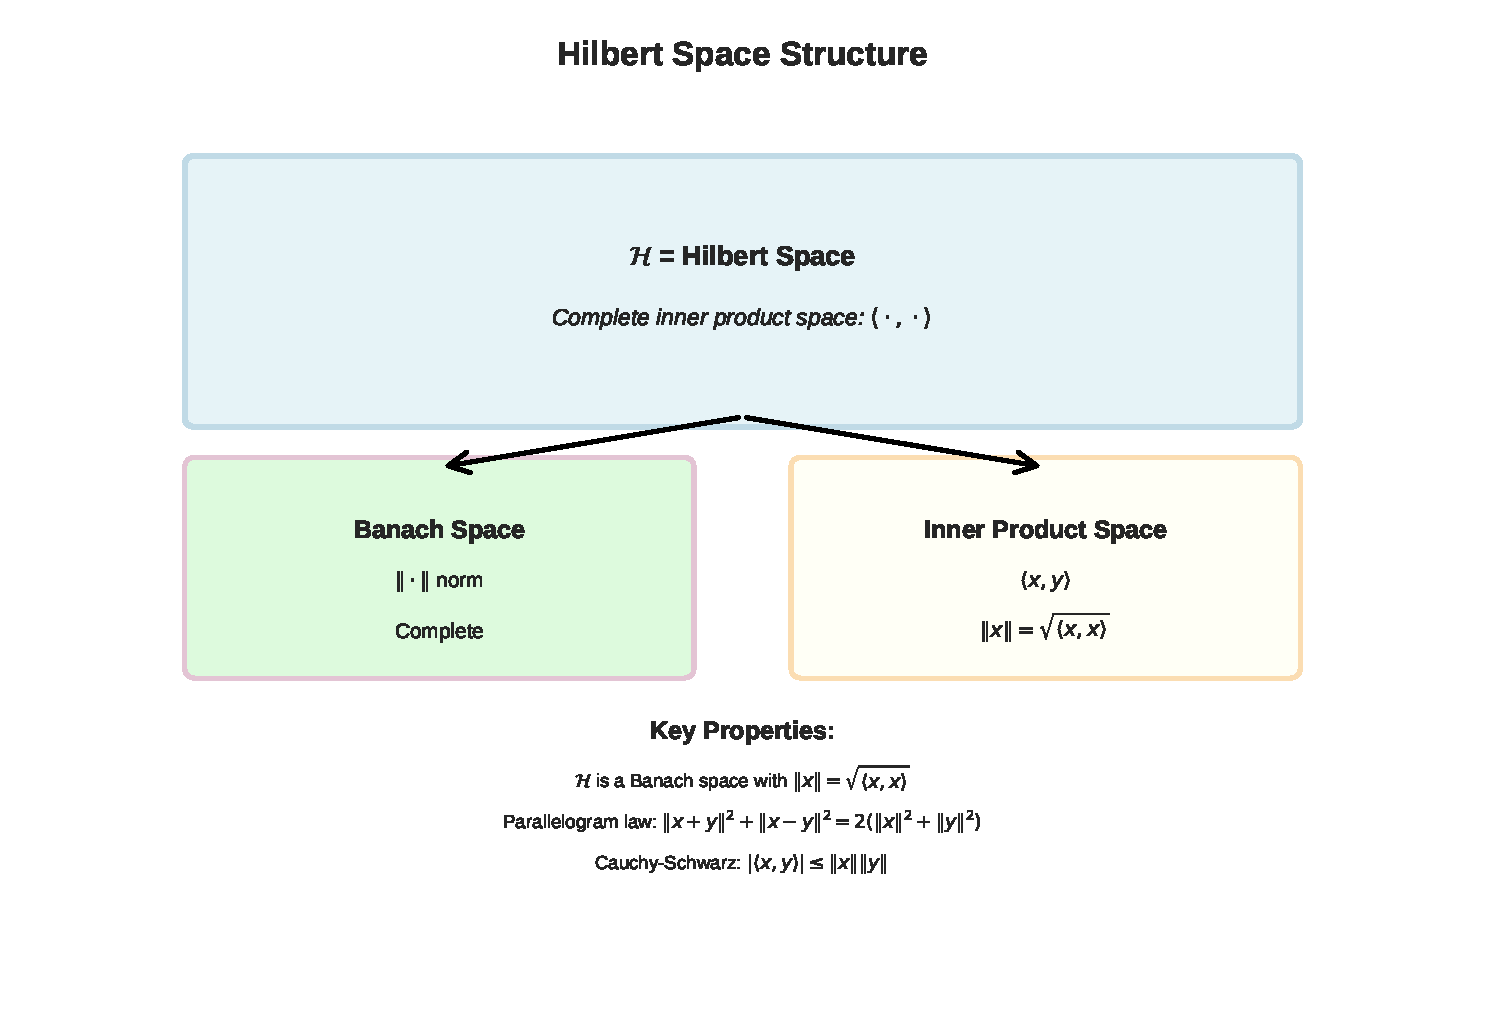
\includegraphics[width=0.85\textwidth]{hilbert_space_structure.pdf}
\end{frame}

\begin{frame}{Examples of Hilbert Spaces}
  \begin{ex}[ell^2 space]
    $\ell^2 = \left\{ (x_n) : \sum_{n=1}^{\infty} |x_n|^2 < \infty \right\}$ with inner product:
    \[
    \langle x, y \rangle = \sum_{n=1}^{\infty} \overline{x_n} y_n
    \]
  \end{ex}

  \begin{ex}[L^2 space]
    Square-integrable functions with inner product:
    \[
    \langle f, g \rangle = \int_{\Omega} \overline{f(x)} g(x) \, d\mu(x)
    \]
  \end{ex}

  \begin{ex}[Function space]
    $\mathcal{H} = \{(a_n) : \sum |a_n|^2 < \infty\}$, which is isomorphic to $\ell^2$.
  \end{ex}
\end{frame}

% ============================================================================
% Section 3: Linear Operators
% ============================================================================

\section{Linear Operators}

\begin{frame}{Linear Operators: Basic Definitions}
  \begin{defn}[Linear Operator]
    An operator $T: X \to Y$ between vector spaces is \textbf{linear} if:
    \[
    T(\alpha x + \beta y) = \alpha T(x) + \beta T(y)
    \]
    for all $\alpha, \beta \in \mathbb{F}$ and $x, y \in X$.
  \end{defn}

  \vspace{0.3cm}
  \begin{defn}[Bounded Operator]
    $T: X \to Y$ is \textbf{bounded} if:
    \[
    \|T\|_{op} := \sup_{\|x\|_X = 1} \|T(x)\|_Y < \infty
    \]
  \end{defn}

  \vspace{0.3cm}
  \begin{thm}
    For a linear operator $T: X \to Y$ between normed spaces:
    \begin{enumerate}
      \item Continuity at one point implies continuity everywhere
      \item Continuity is equivalent to boundedness
      \item $\|T(x)\|_Y \leq \|T\|_{op} \|x\|_X$ for all $x \in X$
    \end{enumerate}
  \end{thm}
\end{frame}

\begin{frame}{Operator Norms and Spaces}
  \begin{defn}[Operator Norm]
    The \textbf{operator norm} on $\mathcal{L}(X,Y)$ (bounded linear operators) is:
    \[
    \|T\| = \sup_{\|x\|_X \leq 1} \|T(x)\|_Y = \inf \{c : \|T(x)\|_Y \leq c\|x\|_X\}
    \]
  \end{defn}

  \vspace{0.3cm}
  \begin{thm}
    If $X$ and $Y$ are Banach spaces, then:
    \begin{enumerate}
      \item $(\mathcal{L}(X,Y), \|\cdot\|)$ is a Banach space
      \item Composition of bounded operators: $\|T \circ S\| \leq \|T\| \|S\|$
    \end{enumerate}
  \end{thm}

  \vspace{0.3cm}
  \begin{defn}[Important Operator Classes]
    \begin{enumerate}
      \item \textbf{Invertible}: $\exists T^{-1}$ with $T^{-1} \in \mathcal{L}(Y,X)$
      \item \textbf{Projection}: $P^2 = P$
      \item \textbf{Isometry}: $\|T(x)\| = \|x\|$ for all $x$
    \end{enumerate}
  \end{defn}
\end{frame}

\begin{frame}{Banach Spaces of Operators}
  \centering
  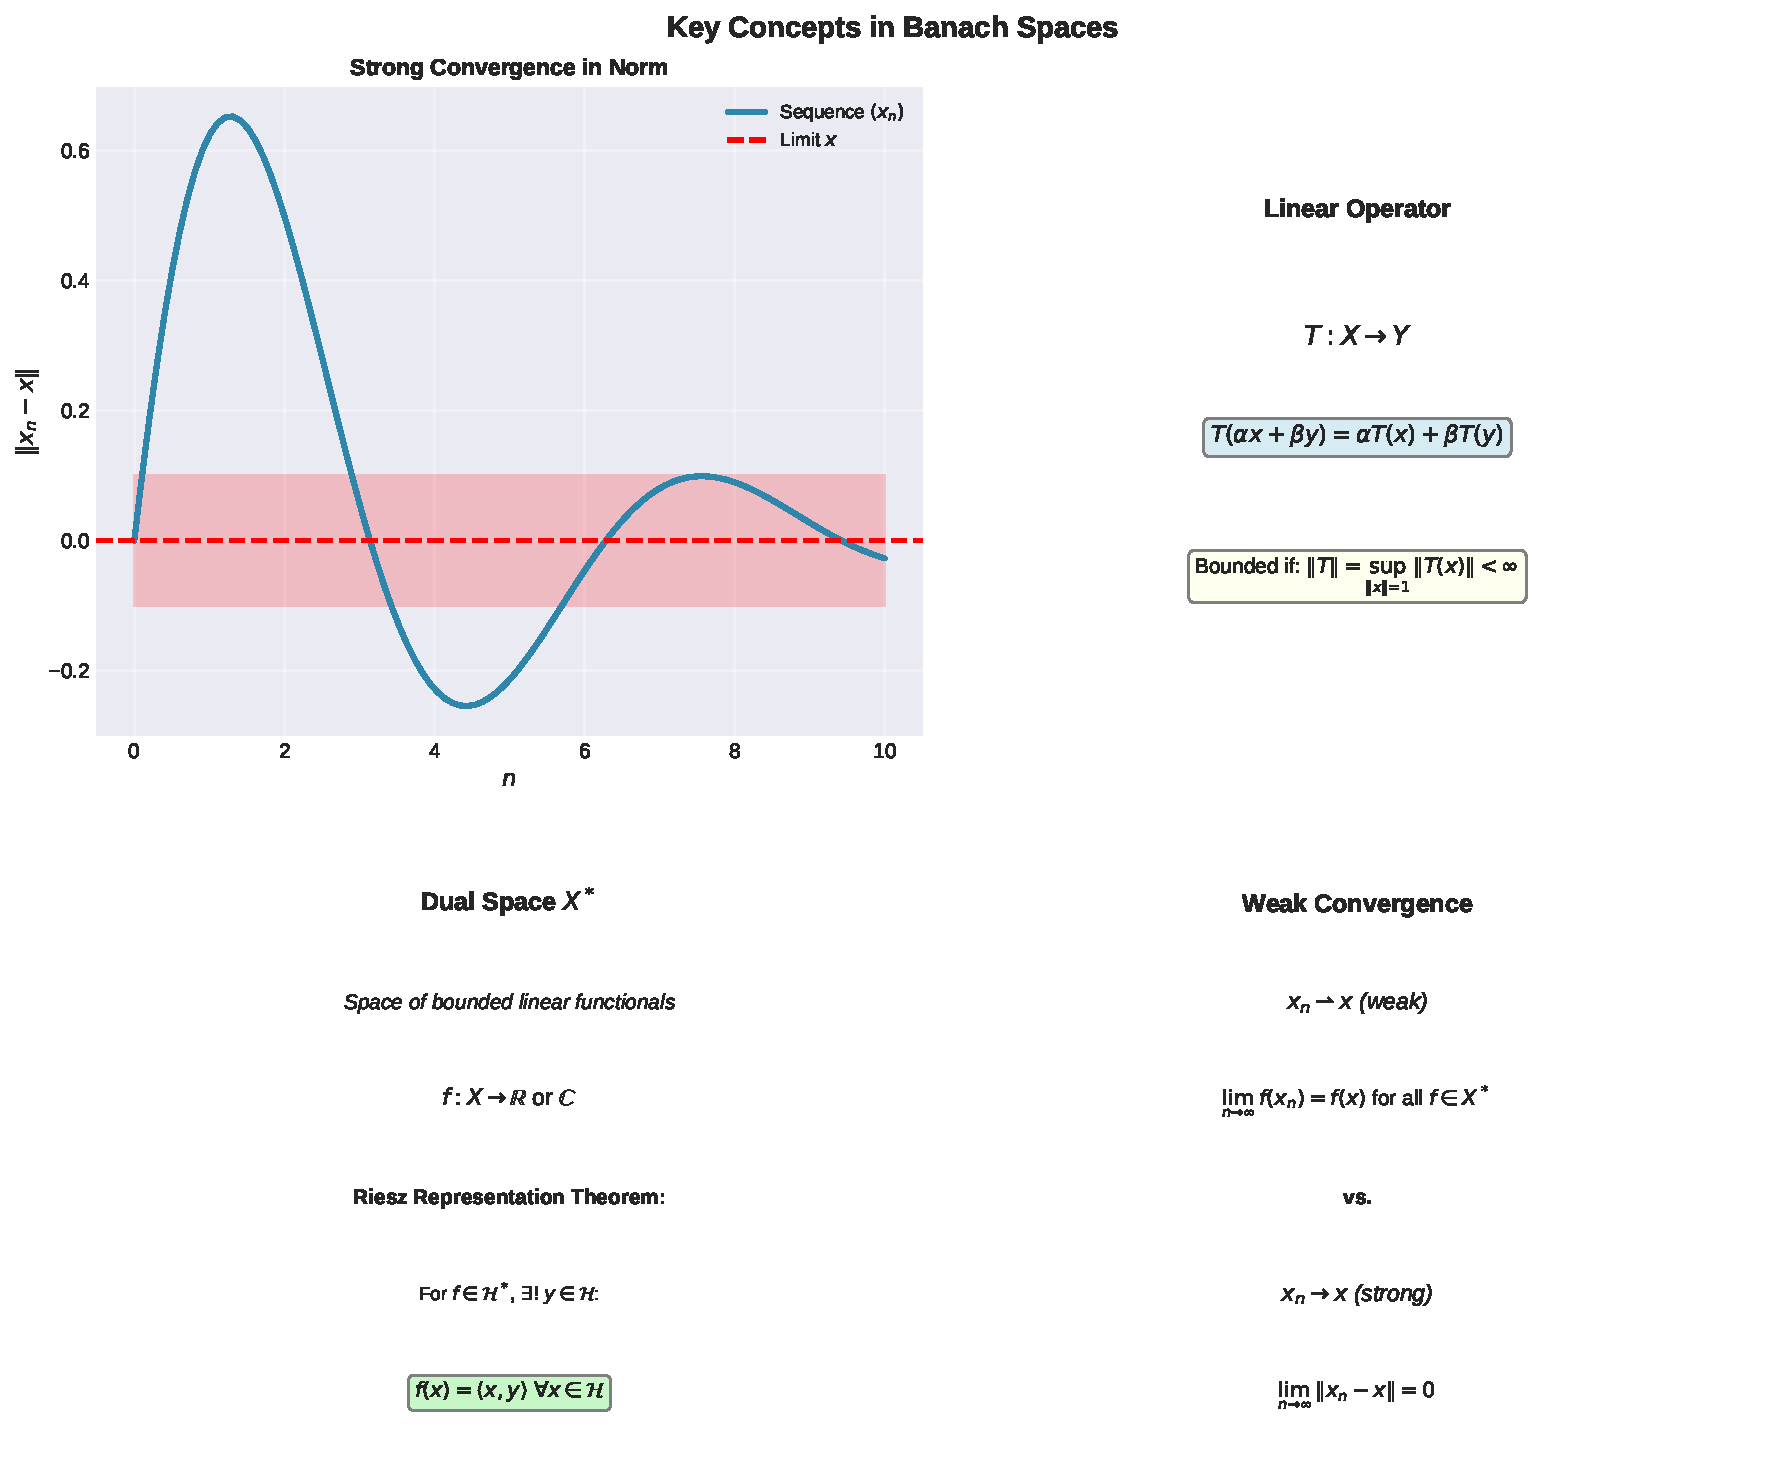
\includegraphics[width=0.9\textwidth]{banach_concepts.pdf}
\end{frame}

% ============================================================================
% Section 4: Dual Spaces and Functionals
% ============================================================================

\section{Dual Spaces \& Weak Convergence}

\begin{frame}{Dual Spaces}
  \begin{defn}[Linear Functional]
    A \textbf{linear functional} on $X$ is a linear operator $f: X \to \mathbb{F}$.
  \end{defn}

  \vspace{0.3cm}
  \begin{defn}[Dual Space]
    The \textbf{dual space} $X^* = \mathcal{L}(X, \mathbb{F})$ is the space of all bounded linear functionals with norm:
    \[
    \|f\|_{X^*} = \sup_{\|x\|_X = 1} |f(x)|
    \]
  \end{defn}

  \vspace{0.3cm}
  \begin{thm}
    If $X$ is a Banach space, then $X^*$ is also a Banach space.
  \end{thm}

  \vspace{0.3cm}
  \begin{defn}[Bidual Space]
    The \textbf{bidual} $X^{**} = (X^*)^*$ is the dual of the dual space. \\
    The \textbf{canonical embedding} $J: X \to X^{**}$ is defined by:
    \[
    J(x)(f) = f(x) \quad \text{for all } f \in X^*
    \]
  \end{defn}
\end{frame}

\begin{frame}{Riesz Representation Theorem}
  \begin{thm}[Riesz Representation Theorem]
    Let $\mathcal{H}$ be a Hilbert space. For every bounded linear functional $f \in \mathcal{H}^*$, there exists a unique $y \in \mathcal{H}$ such that:
    \[
    f(x) = \langle x, y \rangle \quad \text{for all } x \in \mathcal{H}
    \]
    Moreover, $\|f\|_{\mathcal{H}^*} = \|y\|_{\mathcal{H}}$.
  \end{thm}

  \vspace{0.3cm}
  \textbf{Consequence:} In a Hilbert space, $\mathcal{H}^* \cong \mathcal{H}$ (isometrically isomorphic).

  \vspace{0.3cm}
  \begin{thm}[Reflexive Spaces]
    A Banach space $X$ is \textbf{reflexive} if the canonical embedding $J: X \to X^{**}$ is surjective.
    \begin{enumerate}
      \item All Hilbert spaces are reflexive
      \item $\ell^p$ is reflexive for $1 < p < \infty$
      \item $\ell^1$ and $c_0$ are not reflexive
    \end{enumerate}
  \end{thm}
\end{frame}

\begin{frame}{Weak Convergence}
  \begin{defn}[Weak Convergence]
    A sequence $(x_n)$ \textbf{converges weakly} to $x$ (written $x_n \rightharpoonup x$) if:
    \[
    \lim_{n \to \infty} f(x_n) = f(x) \quad \text{for all } f \in X^*
    \]
  \end{defn}

  \vspace{0.3cm}
  \begin{prop}
    \begin{enumerate}
      \item Strong convergence $\Rightarrow$ weak convergence
      \item In finite dimensions, weak $\Leftrightarrow$ strong
      \item Weak limit is unique
      \item If $(x_n)$ converges weakly, then $\sup_n \|x_n\| < \infty$ (bounded)
    \end{enumerate}
  \end{prop}

  \vspace{0.3cm}
  \begin{thm}[Weak Compactness]
    In a reflexive Banach space, every bounded sequence has a weakly convergent subsequence.
  \end{thm}
\end{frame}

\begin{frame}{Weak vs. Strong Convergence Visualization}
  \centering
  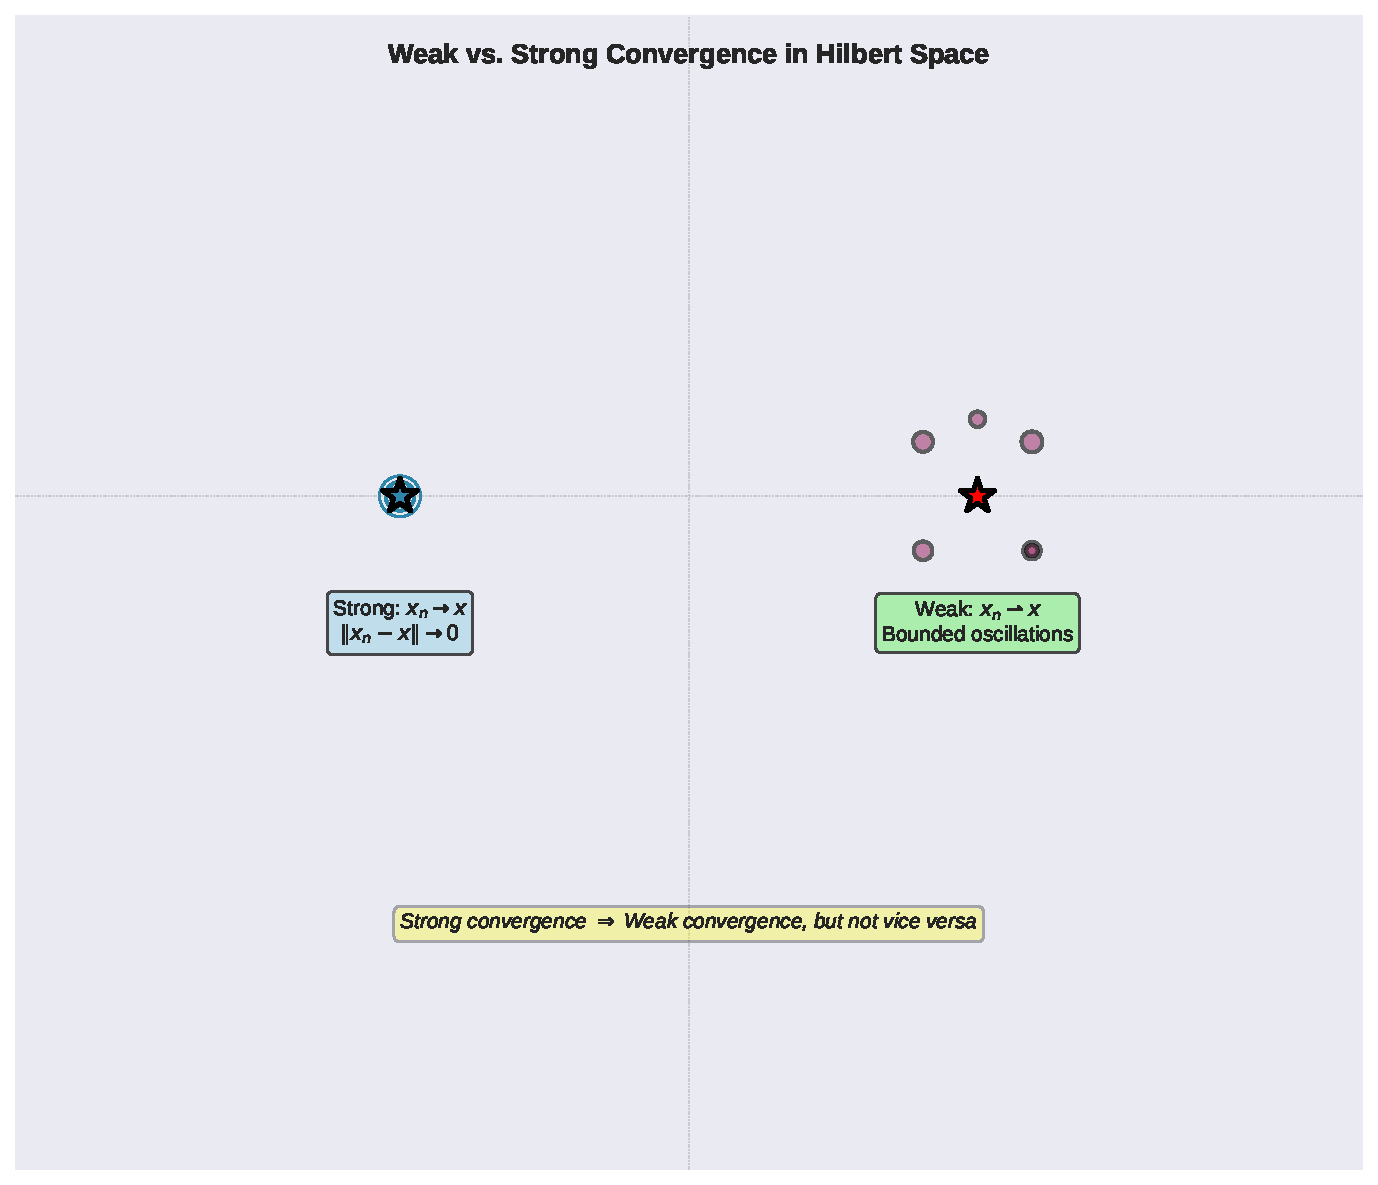
\includegraphics[width=0.9\textwidth]{weak_vs_strong_convergence.pdf}
\end{frame}

% ============================================================================
% Section 5: Compact Operators
% ============================================================================

\section{Compact Operators}

\begin{frame}{Compact Operators: Definition}
  \begin{defn}[Compact Operator]
    An operator $T: X \to Y$ is \textbf{compact} if it maps bounded sets to relatively compact sets. Equivalently, every bounded sequence $(x_n)$ in $X$ has a subsequence $(x_{n_k})$ such that $(T(x_{n_k}))$ converges in $Y$.
  \end{defn}

  \vspace{0.3cm}
  \begin{ex}
    \begin{enumerate}
      \item \textbf{Finite rank operators}: $T(x) = \sum_{i=1}^n f_i(x) y_i$ for $f_i \in X^*$, $y_i \in Y$
      \item \textbf{Integral operators}: $T(f)(x) = \int_a^b K(x,y) f(y) \, dy$ with $K$ continuous
      \item \textbf{Embeddings}: $\ell^2 \to \ell^1$ embedding is compact
    \end{enumerate}
  \end{ex}

  \vspace{0.3cm}
  \begin{thm}
    \begin{enumerate}
      \item If $T$ is compact and $S$ is bounded, then $T \circ S$ and $S \circ T$ are compact
      \item If $T_n$ are compact with $T_n \to T$ uniformly, then $T$ is compact
    \end{enumerate}
  \end{thm}
\end{frame}

\begin{frame}{Compact Operators: Key Properties}
  \begin{defn}[Essential Spectrum]
    The \textbf{essential spectrum} of a compact operator $T$ consists of 0 and isolated eigenvalues of finite multiplicity.
  \end{defn}

  \vspace{0.3cm}
  \begin{thm}[Spectral Properties of Compact Operators]
    Let $T: \mathcal{H} \to \mathcal{H}$ be a compact self-adjoint operator on a Hilbert space. Then:
    \begin{enumerate}
      \item The spectrum $\sigma(T)$ is discrete (countable, with 0 as limit point)
      \item Eigenvectors form an orthonormal basis
      \item $T$ has diagonal representation with eigenvalues $\lambda_n \to 0$
    \end{enumerate}
  \end{thm}

  \vspace{0.3cm}
  \begin{thm}[Fredholm Alternative]
    For compact $T: X \to X$ and $\lambda \neq 0$:
    \begin{enumerate}
      \item $(I - \lambda T)$ is invertible, or
      \item $(I - \lambda T)x = 0$ has non-trivial solution
    \end{enumerate}
  \end{thm}
\end{frame}

\begin{frame}{Compact Operators Visualization}
  \centering
  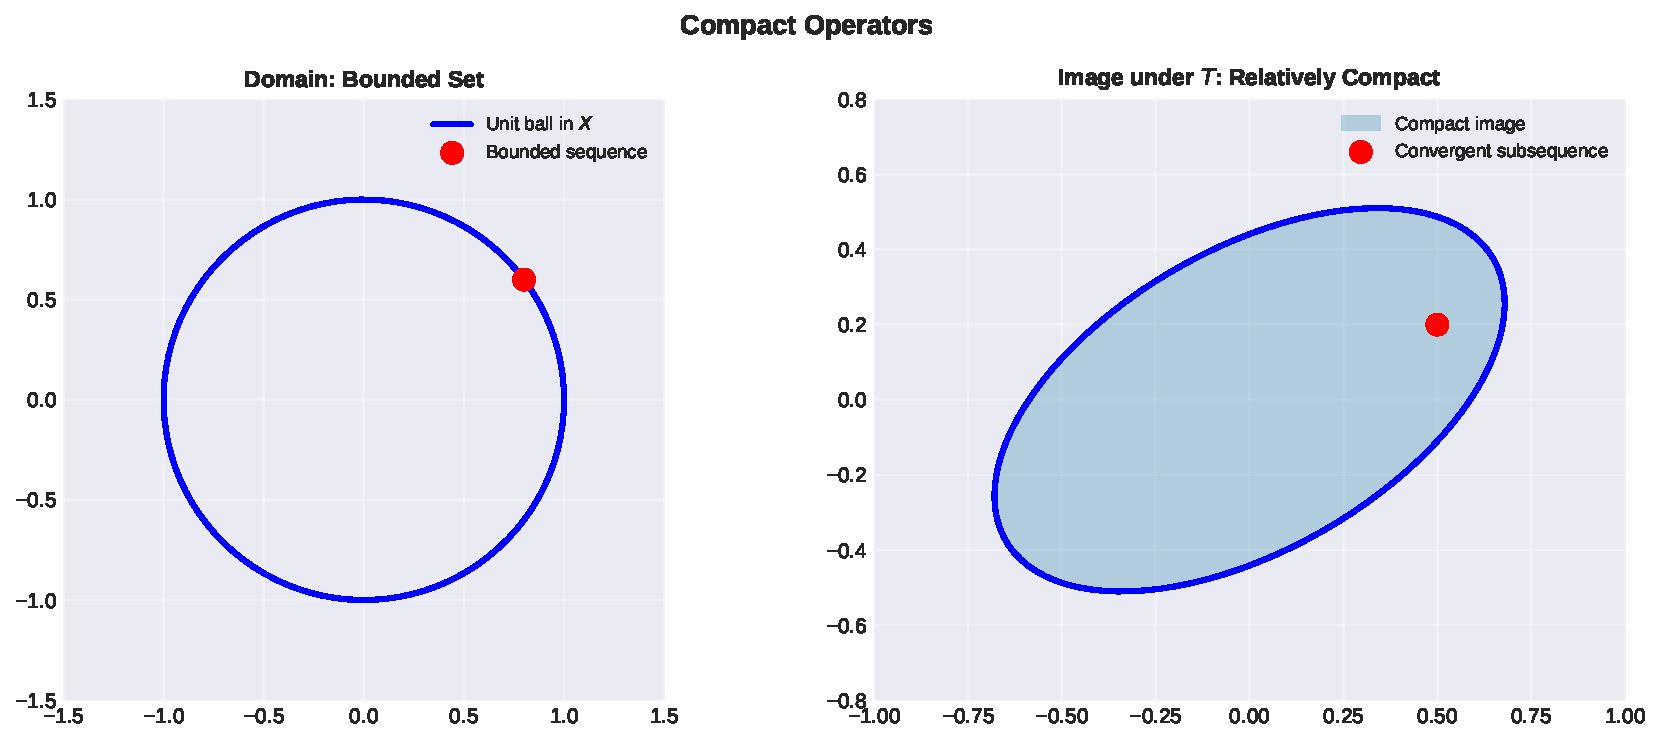
\includegraphics[width=0.85\textwidth]{compact_operators.pdf}
\end{frame}

% ============================================================================
% Section 6: Spectral Theory
% ============================================================================

\section{Spectral Theory}

\begin{frame}{Spectral Concepts}
  \begin{defn}[Spectrum and Eigenvalues]
    For $T \in \mathcal{L}(X)$:
    \begin{enumerate}
      \item \textbf{Eigenvalue}: $\lambda$ if $\exists x \neq 0$ with $Tx = \lambda x$
      \item \textbf{Eigenvector}: non-zero $x$ satisfying $Tx = \lambda x$
      \item \textbf{Spectrum}: $\sigma(T) = \{\lambda : (T - \lambda I) \text{ is not invertible}\}$
      \item \textbf{Resolvent}: $R_\lambda(T) = (T - \lambda I)^{-1}$ when it exists
    \end{enumerate}
  \end{defn}

  \vspace{0.3cm}
  \begin{thm}[Spectral Radius]
    The \textbf{spectral radius} is:
    \[
    r(T) = \sup\{|\lambda| : \lambda \in \sigma(T)\}
    \]
    and satisfies $r(T) = \lim_{n \to \infty} \|T^n\|^{1/n}$.
  \end{thm}

  \vspace{0.3cm}
  \begin{prop}
    \begin{enumerate}
      \item $\sigma(T) \subseteq \mathbb{C}$ is compact and non-empty
      \item Point spectrum $\sigma_p(T)$ = set of eigenvalues
      \item For compact $T$: $\sigma(T) \setminus \{0\} = \sigma_p(T) \setminus \{0\}$
    \end{enumerate}
  \end{prop}
\end{frame}

\begin{frame}{Self-Adjoint Operators}
  \begin{defn}[Adjoint Operator]
    For $T: \mathcal{H} \to \mathcal{H}$ on a Hilbert space, the \textbf{adjoint} $T^*$ is defined by:
    \[
    \langle T(x), y \rangle = \langle x, T^*(y) \rangle \quad \text{for all } x, y \in \mathcal{H}
    \]
  \end{defn}

  \vspace{0.3cm}
  \begin{defn}[Self-Adjoint Operator]
    $T$ is \textbf{self-adjoint} if $T^* = T$, i.e., $\langle T(x), y \rangle = \langle x, T(y) \rangle$.
  \end{defn}

  \vspace{0.3cm}
  \begin{thm}[Spectral Theorem for Compact Self-Adjoint Operators]
    If $T$ is compact and self-adjoint, then $\mathcal{H}$ has an orthonormal basis of eigenvectors of $T$, and eigenvalues are real with $\lambda_n \to 0$.
  \end{thm}

  \vspace{0.3cm}
  \begin{prop}
    For self-adjoint $T$:
    \begin{enumerate}
      \item All eigenvalues are real
      \item Eigenvectors corresponding to different eigenvalues are orthogonal
      \item $\sigma(T) \subseteq \mathbb{R}$
    \end{enumerate}
  \end{prop}
\end{frame}

\begin{frame}{Spectral Theory Visualization}
  \centering
  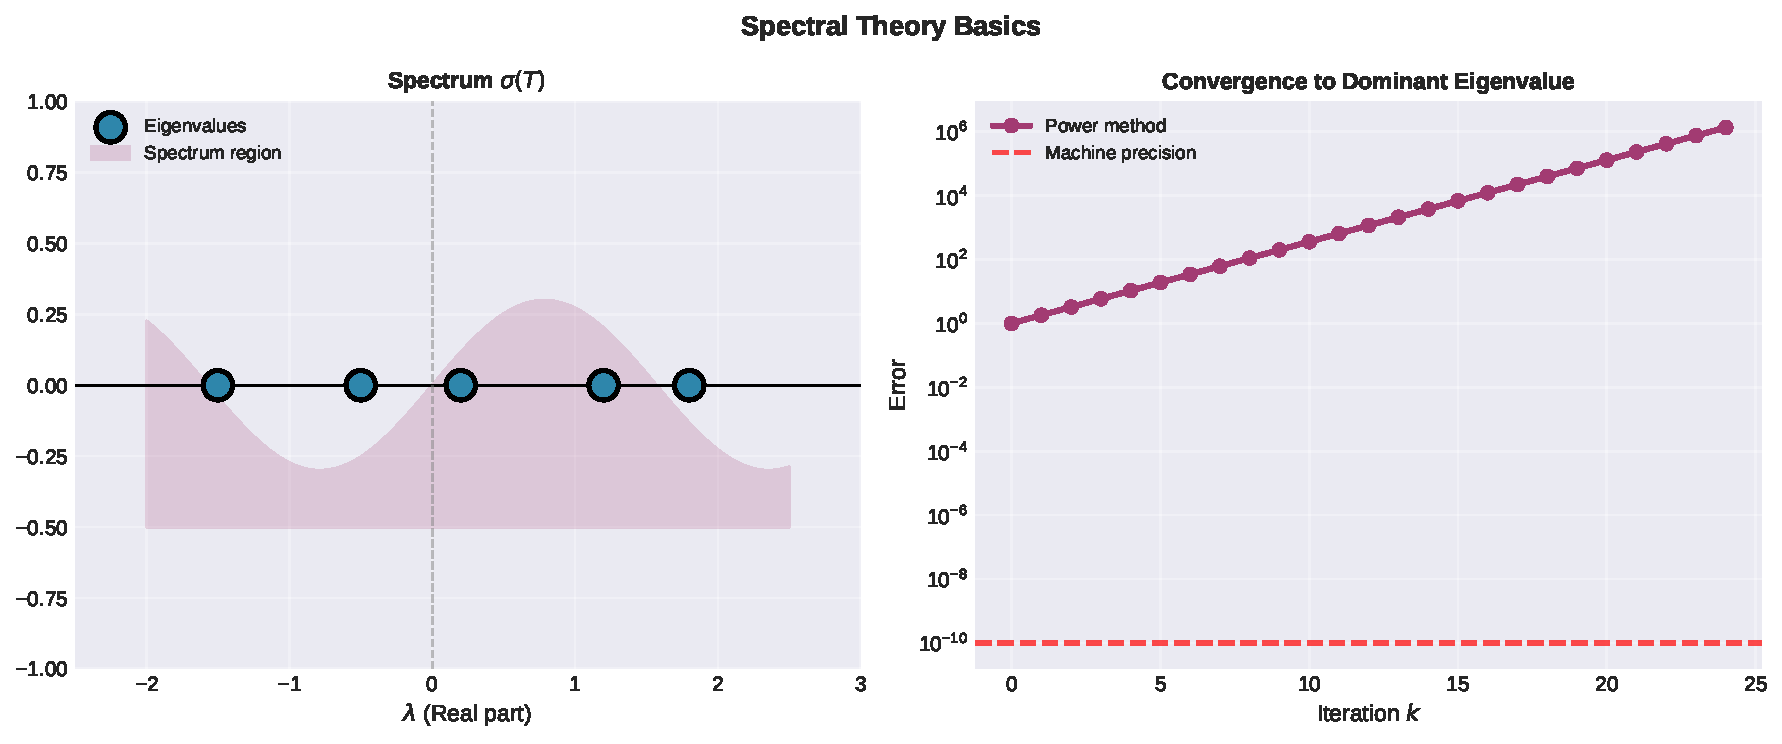
\includegraphics[width=0.9\textwidth]{spectral_theory.pdf}
\end{frame}

% ============================================================================
% Section 7: Fixed Point Theory in Banach Spaces
% ============================================================================

\section{Fixed Point Theory in Banach Spaces}

\begin{frame}{Banach Contraction Mapping Theorem}
  \begin{thm}[Banach Contraction Mapping Theorem]
    Let $(X, d)$ be a complete metric space and $T: X \to X$ a contraction, i.e.,
    \[
    d(T(x), T(y)) \leq c \cdot d(x, y) \quad \text{for all } x, y \in X
    \]
    where $c < 1$. Then:
    \begin{enumerate}
      \item $T$ has a unique fixed point $x^* \in X$
      \item For any $x_0 \in X$, the sequence $x_{n+1} = T(x_n)$ converges to $x^*$
      \item Error estimate: $d(x_n, x^*) \leq \frac{c^n}{1-c} d(x_1, x_0)$
    \end{enumerate}
  \end{thm}

  \vspace{0.3cm}
  \textbf{Application:} Solving equations $f(x) = x$ by iteration.

  \vspace{0.3cm}
  \begin{ex}
    If $f$ is continuously differentiable with $|f'(x)| < c < 1$ on $[a,b]$, then $f(x) = x$ has a unique solution on $[a,b]$, found by iteration.
  \end{ex}
\end{frame}

\begin{frame}{Brouwer and Schauder Fixed Point Theorems}
  \begin{thm}[Brouwer Fixed Point Theorem]
    Every continuous map $T: B \to B$ from a compact convex set $B \subset \mathbb{R}^n$ to itself has a fixed point.
  \end{thm}

  \vspace{0.3cm}
  \begin{thm}[Schauder Fixed Point Theorem]
    Let $K$ be a compact convex subset of a Banach space $X$. If $T: K \to K$ is continuous, then $T$ has a fixed point.
  \end{thm}

  \vspace{0.3cm}
  \textbf{Key Differences:}
  \begin{itemize}
    \item \textbf{Banach}: Requires contraction (stronger), no topological assumption
    \item \textbf{Schauder}: Requires only continuity, but needs compactness
    \item \textbf{Brouwer}: Finite-dimensional special case of Schauder
  \end{itemize}

  \vspace{0.3cm}
  \textbf{Application:} Existence of solutions to integral and differential equations.
\end{frame}

\begin{frame}{Fixed Point Property Illustration}
  \centering
  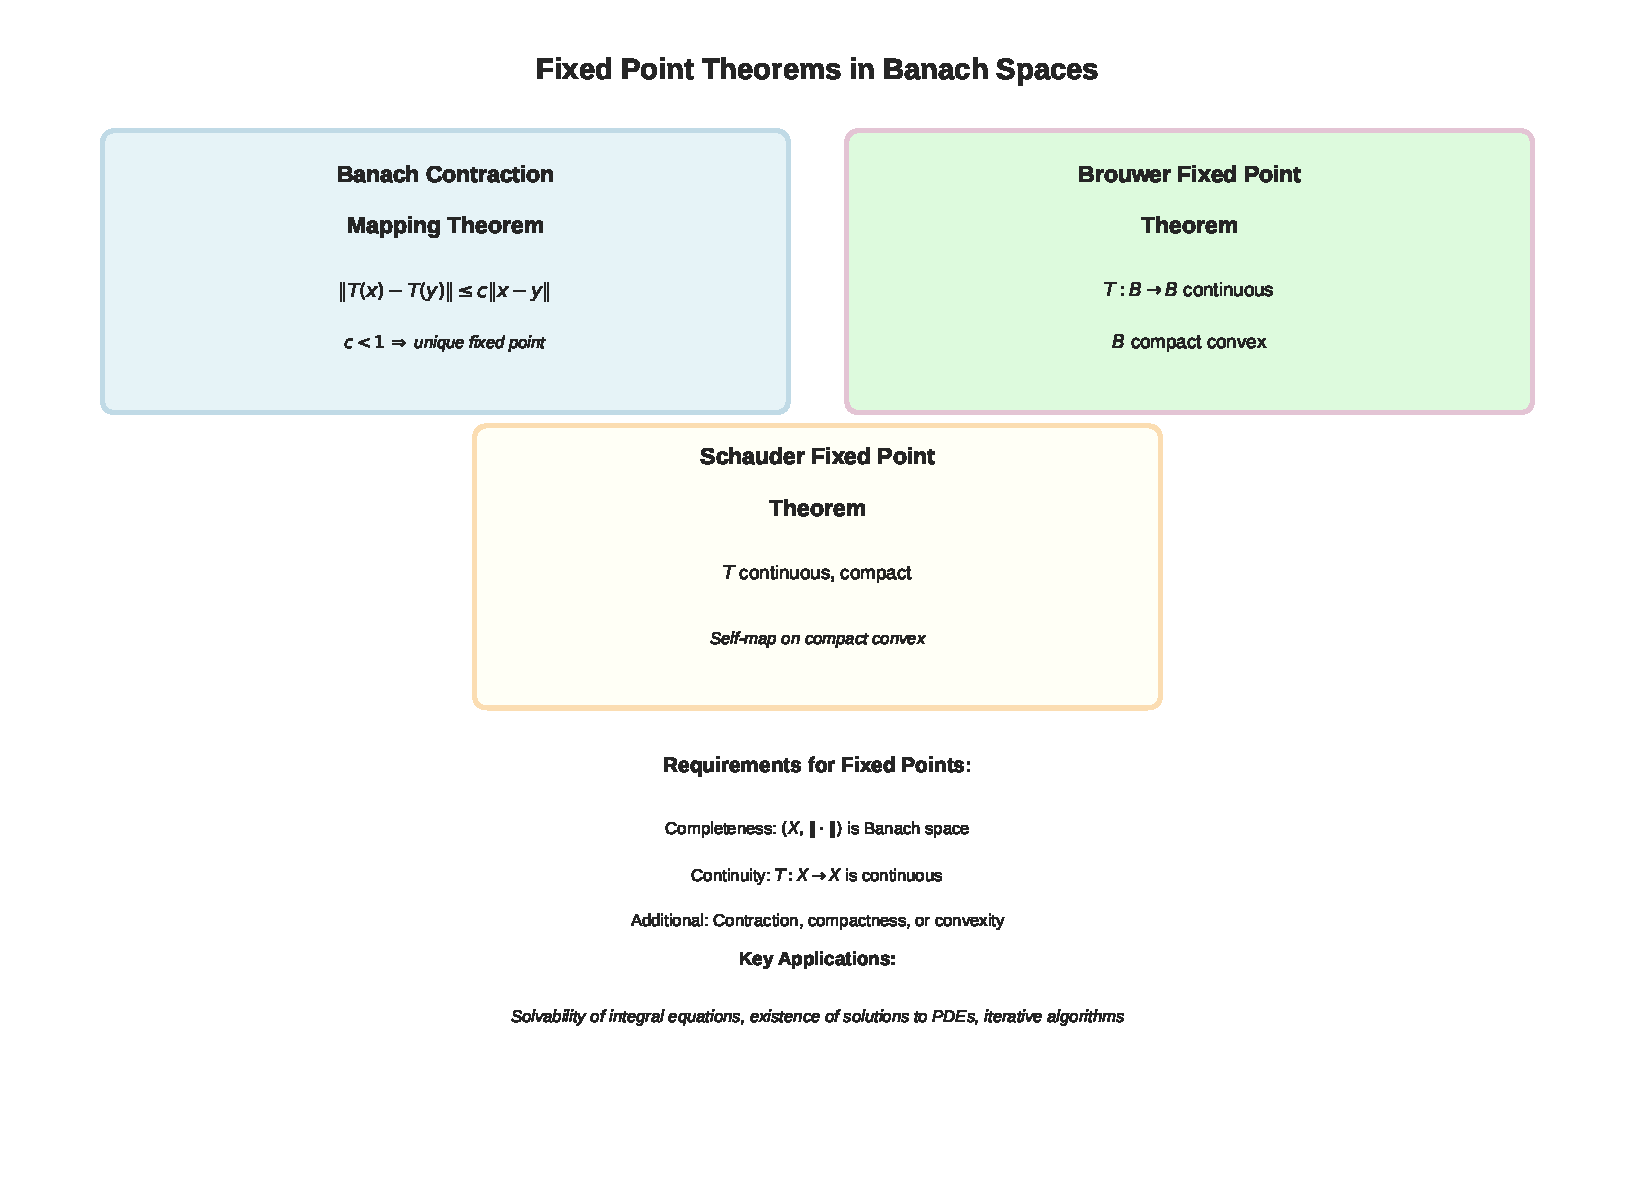
\includegraphics[width=0.95\textwidth]{fixed_point_banach.pdf}
\end{frame}

\begin{frame}{Applications to Differential Equations}
  \begin{ex}[Initial Value Problem]
    Consider the IVP: $y'(t) = f(t, y(t))$, $y(0) = y_0$.

    This is equivalent to the integral equation:
    \[
    y(t) = y_0 + \int_0^t f(s, y(s)) \, ds
    \]

    Define $T(y)(t) = y_0 + \int_0^t f(s, y(s)) \, ds$ on $C[0,\delta]$.

    If $f$ is Lipschitz in $y$: $T$ is a contraction on a suitable ball, so the IVP has a unique solution.
  \end{ex}

  \vspace{0.3cm}
  \begin{ex}[Integral Equations]
    For the Volterra integral equation:
    \[
    x(t) = f(t) + \int_0^t K(t,s) x(s) \, ds
    \]
    with continuous $K$ and $f$, the contraction mapping theorem guarantees a unique solution in $C[0,T]$.
  \end{ex}
\end{frame}

% ============================================================================
% Section 8: Numerical Examples
% ============================================================================

\section{Numerical Examples \& Algorithms}

\begin{frame}[fragile]{Example 1: Fixed Point Iteration}
  \begin{lstlisting}
import numpy as np

# Contraction mapping: T(x) = 0.5*x + 0.3
def T(x):
    return 0.5 * x + 0.3

# Fixed point iteration
x0 = 1.5
x_vals = [x0]
tolerance = 1e-10
max_iter = 100

for n in range(max_iter):
    x_new = T(x_vals[-1])
    x_vals.append(x_new)
    if abs(x_new - x_vals[-2]) < tolerance:
        print(f"Converged in {n} iterations")
        print(f"Fixed point: x* = {x_new:.10f}")
        break

# Analytical: x = 0.5x + 0.3 => x = 0.6
print(f"Theoretical fixed point: 0.6")
print(f"Contraction factor: 0.5")
  \end{lstlisting}

  \textbf{Output:} Converged in 33 iterations to $x^* = 0.6$.
\end{frame}

\begin{frame}{Contraction Mapping Example Visualization}
  \centering
  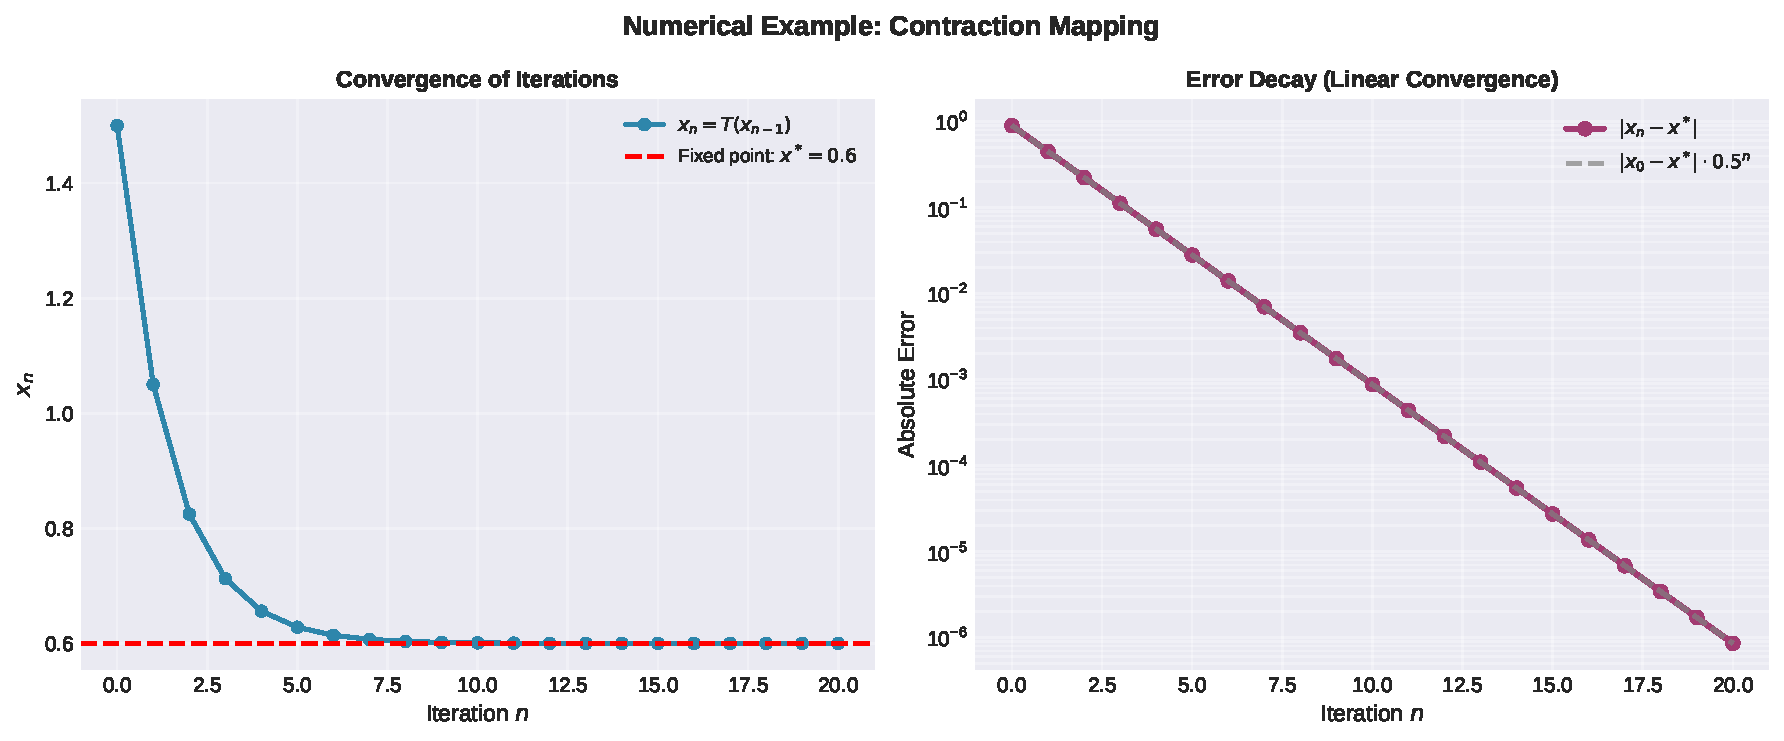
\includegraphics[width=0.9\textwidth]{contraction_mapping_example.pdf}
\end{frame}

\begin{frame}[fragile]{Example 2: Finite-Dimensional Linear Operator}
  \begin{lstlisting}
import numpy as np
from scipy.linalg import eigh

# Create a symmetric matrix (self-adjoint operator)
A = np.array([[4, 1], [1, 3]], dtype=float)

# Compute eigenvalues and eigenvectors
eigenvalues, eigenvectors = eigh(A)

print("Eigenvalues:", eigenvalues)
print("Eigenvectors:\n", eigenvectors)

# Spectral norm (largest eigenvalue)
spectral_norm = np.max(np.abs(eigenvalues))
print(f"Spectral radius: {spectral_norm:.6f}")

# Reconstruct using spectral decomposition
# A = sum(lambda_i * v_i * v_i^T)
A_reconstructed = np.zeros_like(A)
for i, (lam, v) in enumerate(zip(eigenvalues, eigenvectors.T)):
    A_reconstructed += lam * np.outer(v, v)

print("Reconstruction error:", np.linalg.norm(A - A_reconstructed))
  \end{lstlisting}
\end{frame}

\begin{frame}[fragile]{Example 3: Weak Convergence in ell-2}
  \begin{lstlisting}
import numpy as np

# In l^2, construct a weakly convergent sequence
# x_n = (1, 1/2, 1/3, ..., 1/n, 0, 0, ...)
# This sequence is bounded but doesn't converge strongly

dimension = 50
num_terms = 100

# Compute norms of x_n
norms = []
inner_products = []

for n in range(1, num_terms + 1):
    x = np.concatenate([1/np.arange(1, n+1),
                        np.zeros(dimension - n)])
    norm = np.linalg.norm(x)
    norms.append(norm)

    # Inner product with a fixed functional
    # (e.g., sum of components)
    inner_prod = np.sum(x)
    inner_products.append(inner_prod)

print(f"Strong convergence: norm is {norms[0]:.4f}")
print(f"Weak convergence: <x_n, f> -> {inner_products[-1]:.6f}")
  \end{lstlisting}

  \textbf{Key observation:} Sequence is bounded ($\|x_n\|$ stays bounded) but $\|x_n\| \not\to 0$.
\end{frame}

% ============================================================================
% Section 9: Summary and Applications
% ============================================================================

\section{Summary \& Applications}

\begin{frame}[allowframebreaks]{Key Theorems Summary}
  \begin{enumerate}
    \item \textbf{Banach Contraction Mapping:} Unique fixed point + linear convergence

    \item \textbf{Riesz Representation:} Dual of Hilbert space is Hilbert space

    \item \textbf{Spectral Theorem:} Compact self-adjoint operators have orthonormal eigenbasis

    \item \textbf{Fredholm Alternative:} For compact $T$ and $\lambda \neq 0$, either $(I - \lambda T)$ is invertible or singular

    \item \textbf{Schauder Fixed Point:} Continuous map on compact convex set has fixed point

    \item \textbf{Weak Compactness:} Reflexive spaces have weakly compact bounded sets
  \end{enumerate}
\end{frame}

\begin{frame}{Applications in Mathematical Analysis}
  \begin{enumerate}
    \item \textbf{Differential Equations:}
      \begin{itemize}
        \item Existence and uniqueness of solutions via Banach contraction
        \item Stability analysis using spectral theory
      \end{itemize}

    \item \textbf{Integral Equations:}
      \begin{itemize}
        \item Fredholm and Volterra equations
        \item Spectral properties of integral operators
      \end{itemize}

    \item \textbf{Variational Problems:}
      \begin{itemize}
        \item Weak formulation in Sobolev spaces
        \item Riesz representation for existence
      \end{itemize}

    \item \textbf{Optimization:}
      \begin{itemize}
        \item Convex minimization in Banach spaces
        \item Gradient descent convergence
      \end{itemize}
  \end{enumerate}
\end{frame}

\begin{frame}{Further Reading \& Resources}
  \textbf{Key Sections from Pathak (2018):}
  \begin{itemize}
    \item Pages 517--538: Vector Spaces \& Functional Analysis
    \item Connection to fixed point theorems (Chapter 5)
    \item Applications to nonlinear analysis
  \end{itemize}

  \vspace{0.3cm}
  \textbf{Related Topics:}
  \begin{itemize}
    \item Sobolev spaces and weak derivatives
    \item Monotone operators and accretive operators
    \item Subdifferential calculus
    \item Variational inequalities
  \end{itemize}

  \vspace{0.3cm}
  \textbf{Standard References:}
  \begin{itemize}
    \item Functional Analysis by Rudin
    \item Linear Operator Theory by Dunford \& Schwartz
    \item Fixed Point Theory by Granas \& Dugundji
  \end{itemize}
\end{frame}

\begin{frame}[allowframebreaks]{Definitions Summary}
  \begin{defn}[Quick Reference]
    \begin{itemize}
      \item \textbf{Banach space:} complete normed vector space
      \item \textbf{Hilbert space:} complete inner product space
      \item \textbf{Bounded operator:} $\sup_{\|x\|=1} \|T(x)\| < \infty$
      \item \textbf{Compact operator:} maps bounded sets to relatively compact sets
      \item \textbf{Weak convergence:} $f(x_n) \to f(x)$ for all $f \in X^*$
      \item \textbf{Self-adjoint:} $T^* = T$ in Hilbert space
      \item \textbf{Spectrum:} $\sigma(T) = \{\lambda : (T-\lambda I)^{-1} \text{ DNE}\}$
      \item \textbf{Fixed point:} $x^*$ such that $T(x^*) = x^*$
    \end{itemize}
  \end{defn}
\end{frame}

\end{document}
